%---------------------------------------------------------------------
%
%    Project Name: Radar System Signal Process Software Design Discuss
%
%---------------------------------------------------------------------
%
%               created by LuoMin <luomin5417@gmail.com>
%
%                       Last-modified: 2018-12-14
%
%---------------------------------------------------------------------

\documentclass[a4paper,12pt]{report}
\usepackage{etex}
\usepackage{ctex}
%\usepackage{xeCJK}
\usepackage{times}
\usepackage{setspace}
\usepackage{fancyhdr}
\usepackage{graphicx}
\usepackage{wrapfig}
\usepackage{array}  
\usepackage{fontspec,xunicode,xltxtra}
\usepackage{titlesec}
\usepackage{titletoc}
\usepackage[titletoc]{appendix}
\usepackage[top=30mm,bottom=30mm,left=20mm,right=20mm]{geometry}
\usepackage{cite}
\usepackage{listings}
\usepackage{caption,subcaption}
\usepackage[framed,numbered,autolinebreaks,useliterate]{mcode} % 插入代码
\usepackage{xeboiboites}
\usepackage{amsmath,amssymb}
\usepackage{hyperref}
\usepackage{float}

\usepackage{xcolor}
\usepackage{tcolorbox}

\usepackage{enumerate}
\usepackage[font=small,labelsep=space]{caption}
\usepackage{multirow}

\RequirePackage{tkz-network}

\hypersetup{hidelinks}

\XeTeXlinebreaklocale "zh"
\XeTeXlinebreakskip = 0pt plus 1pt minus 0.1pt

%---------------------------------------------------------------------
%	页眉页脚设置
%---------------------------------------------------------------------
\fancypagestyle{plain}{
    \pagestyle{fancy}      %改变章节首页页眉
}

\pagestyle{fancy}
\lhead{\kaishu~宜通华盛~}
\rhead{\kaishu~研发部~}
\cfoot{\thepage}

%---------------------------------------------------------------------
%	章节标题设置
%---------------------------------------------------------------------
\titleformat{\chapter}{\centering\zihao{-1}\heiti}{第\chinese{chapter}章}{1em}{}
\titlespacing{\chapter}{0pt}{*0}{*6}

%---------------------------------------------------------------------
%	摘要标题设置
%---------------------------------------------------------------------
\renewcommand{\abstractname}{\zihao{-3} 摘\quad 要}

%---------------------------------------------------------------------
%	参考文献设置
%---------------------------------------------------------------------
\renewcommand{\bibname}{\zihao{2}{\hspace{\fill}参\hspace{0.5em}考\hspace{0.5em}文\hspace{0.5em}献\hspace{\fill}}}

%---------------------------------------------------------------------
%	引用文献设置为上标
%---------------------------------------------------------------------
\makeatletter
\def\@cite#1#2{\textsuperscript{[{#1\if@tempswa , #2\fi}]}}
\makeatother

%---------------------------------------------------------------------
%	目录页设置
%---------------------------------------------------------------------
\titlecontents{chapter}[0em]{\songti\zihao{-4}}{\thecontentslabel\ }{}
{\hspace{.5em}\titlerule*[4pt]{$\cdot$}\contentspage}
\titlecontents{section}[2em]{\vspace{0.1\baselineskip}\songti\zihao{-4}}{\thecontentslabel\ }{}
{\hspace{.5em}\titlerule*[4pt]{$\cdot$}\contentspage}
\titlecontents{subsection}[4em]{\vspace{0.1\baselineskip}\songti\zihao{-4}}{\thecontentslabel\ }{}
{\hspace{.5em}\titlerule*[4pt]{$\cdot$}\contentspage}

%---------------------------------------------------------------------
%	公式设置
%---------------------------------------------------------------------
%%define the newthem environment
\newboxedtheorem[small box style={fill=blue!20,draw=black, 
    rounded corners},
    big box style={fill=blue!10,draw=orange,thick,rounded corners},
    headfont=\bfseries]%
    {proposition}{公式}{somecounter} 

%---------------------------------------------------------------------
%   生成大纲
%---------------------------------------------------------------------

\begin{document}
%---------------------------------------------------------------------
%	封面设置
%---------------------------------------------------------------------
\begin{titlepage}
    \begin{center}
        
    
\includegraphics[width=0.8\textwidth]{figure//etws.png}\\
    \vspace{40mm}
    \textbf{\zihao{2}\kaishu{ETWS-1810雷达信处}}\\[0.8cm]
    \textbf{\zihao{2}\kaishu{软件设计讨论}}\\[3cm]
    
    \vspace{\fill}
    
\setlength{\extrarowheight}{3mm}
{\songti\zihao{3}	
\begin{tabular}{rl}
    
    {\makebox[5\ccwd][s]{部\qquad 门:}}& ~\kaishu 研发部\\
    
    {\makebox[5\ccwd][s]{编\qquad 制:}}& ~\kaishu 罗敏 \\ 

    {\makebox[5\ccwd][s]{版\qquad 本:}}& ~\kaishu 1.0 \\

\end{tabular}
 }\\[2cm]
\vspace{\fill}
\zihao{4}
使用\LaTeX 撰写于\today
    \end{center}	
\end{titlepage}

%---------------------------------------------------------------------
%  摘要页
%---------------------------------------------------------------------
\begin{abstract}
\begin{spacing}{1.5}
    {\zihao{-4}
    本文主要是关于雷达系统自研信号处理分系统软件设计讨论,目的是确定信号处理分系统软件和
    算法处理部分的详细工作。因对于信号处理部分均是从零起步,一个好的实现方案和计划更显的
    尤为重要,本文从信号处理分系统输出目标出发,逐步详细阐述各个设计目标的计算和实现过程。

    \textbf{关键字}:\quad 雷达系统 \quad 信号处理 \quad 算法 \quad 实现
    }
\end{spacing}
\end{abstract}

%---------------------------------------------------------------------
%  目录页
%---------------------------------------------------------------------
\tableofcontents % 生成目录

%---------------------------------------------------------------------
%  第一章
%---------------------------------------------------------------------
\chapter{设计目标}
\setcounter{page}{1}
\begin{spacing}{1.5}
\songti\zihao{-4}

\section{输出指标}
本节主要是对雷达信号处理分系统的设计指标进行确认,确定设计输出的指标之后,才能够更好的针
对设计指标进行软件设计和规划。
\begin{figure}[hbtp]
    \centering
    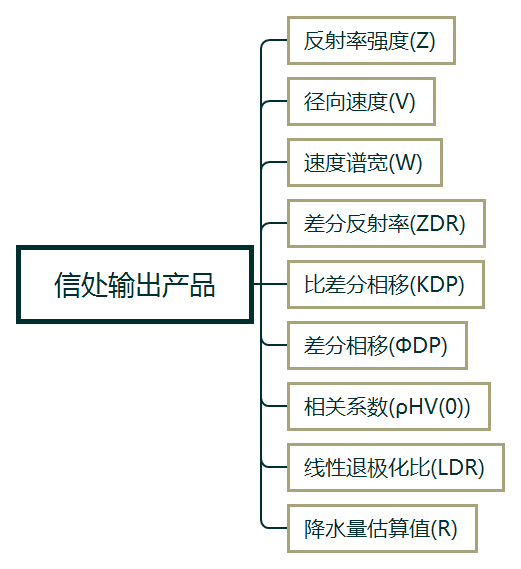
\includegraphics [width=0.5\textwidth]{figure//output.png}
    \caption{信处输出原始产品}\label{output}
\end{figure}
在图1.1中根据《X波段双偏振天气雷达改造升级项目立项报告》列了一下信处分系统应该要输出的原
始产品。


\section{硬件架构}
目前硬件架构已经基本确认,具体如图1.2所示主要采用AD板+接口板+X86板的方案。AD板与接口板
之间采用SIRO接口连接,接口板与X86板之间采用PCIe3.0接口连接。如图所示,AD板主要负责下变
频、抽取、滤波等工作,接口板则负责接收AD板采集的数据,然后对数据进行DBF、脉冲压缩等处理,
同时需要控制伺服、波控等组件,X86板则接收接口板处理后的数据做后半段的信号数据处理,最终输
出上一节中提到的输出指标。
\begin{figure}[hbtp]
    \centering
    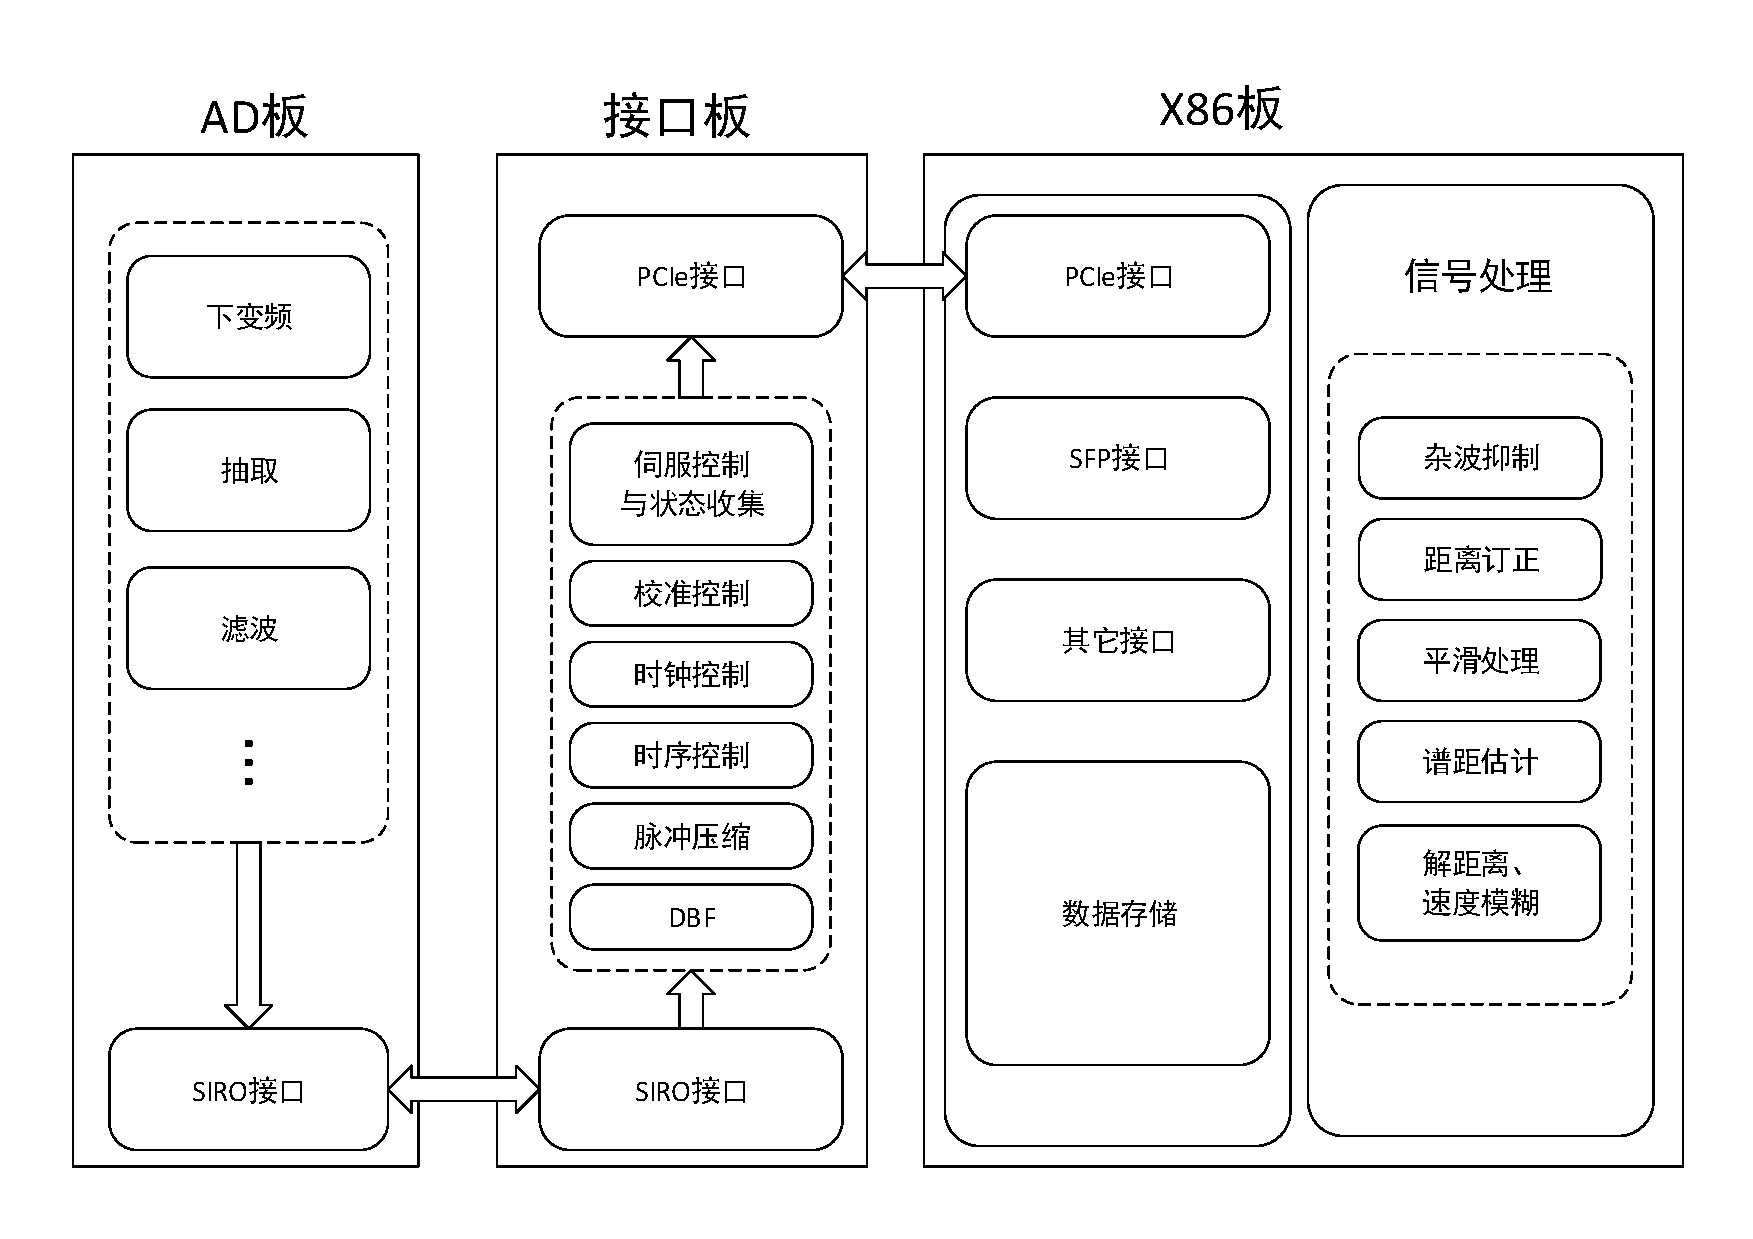
\includegraphics [width=0.8\textwidth]{figure//HardDesign.pdf}
    \caption{硬件设计}\label{HardDesign}
\end{figure}

因本文主要讨论软件的设计实现,主要会聚焦于X86板的信号处理部分,目前接口板与X86板的数据通
道已经是对接过,可以从接口板读取相关数据,后续的工作便是两个主要的工作:
\begin{itemize}
    \itemsep=3pt
    \parskip=0pt
    \setlength{\itemindent}{1em}
    \item 设计接口板与X86板接收数据的协议
    \item 处理理接收到的数据
\end{itemize}


%\begin{table}[hbtp]
%	\centering
%	\caption{软件功能要求}
%	\begin{tabular}{lp{3cm}p{4cm}p{4cm}}
%	\hline
%	模块    & 软件            & 功能                 &         备注\\
%	\hline
%    \multirow{2}{*}{网关}     & 系统软件& 网关的基本通信功能& 基于Openwrt开源系统\\
%    %\cline{2-4}
%	~  & 远程控制软件    & 设备远程配置       & 基于curl工具进行开发\\
%    %\hline
%
%    服务器  & 服务器软件  & 采集数据建立通信通道 & 定制开发\\
%    %\hline          
%
%	管理软件    & 设备管理软件 & 管理网关和设备     & 使用浏览器远程登录服务器 \\
%	\hline          
%	\end{tabular}
%	\label{tab:Cost_evalua}
%\end{table}

\end{spacing}

%---------------------------------------------------------------------
%  第二章
%---------------------------------------------------------------------
\chapter{设计原理}
\begin{spacing}{1.5}
\songti\zihao{-4}

\section{数据模型}
\subsection{三维数据模型}
需要对雷达回波进行数据处理,首先要将回波数据抽象成一个数据处理模型,在这里采用了三维数据
块作为一个数据处理模型\cite{FundamentalsOfRadarSignalProcessing},这一处理方法引用自
雷达信号处理基础第三章,基本处理模型如图2.1所示:
\begin{figure}[hbtp]
    \centering
    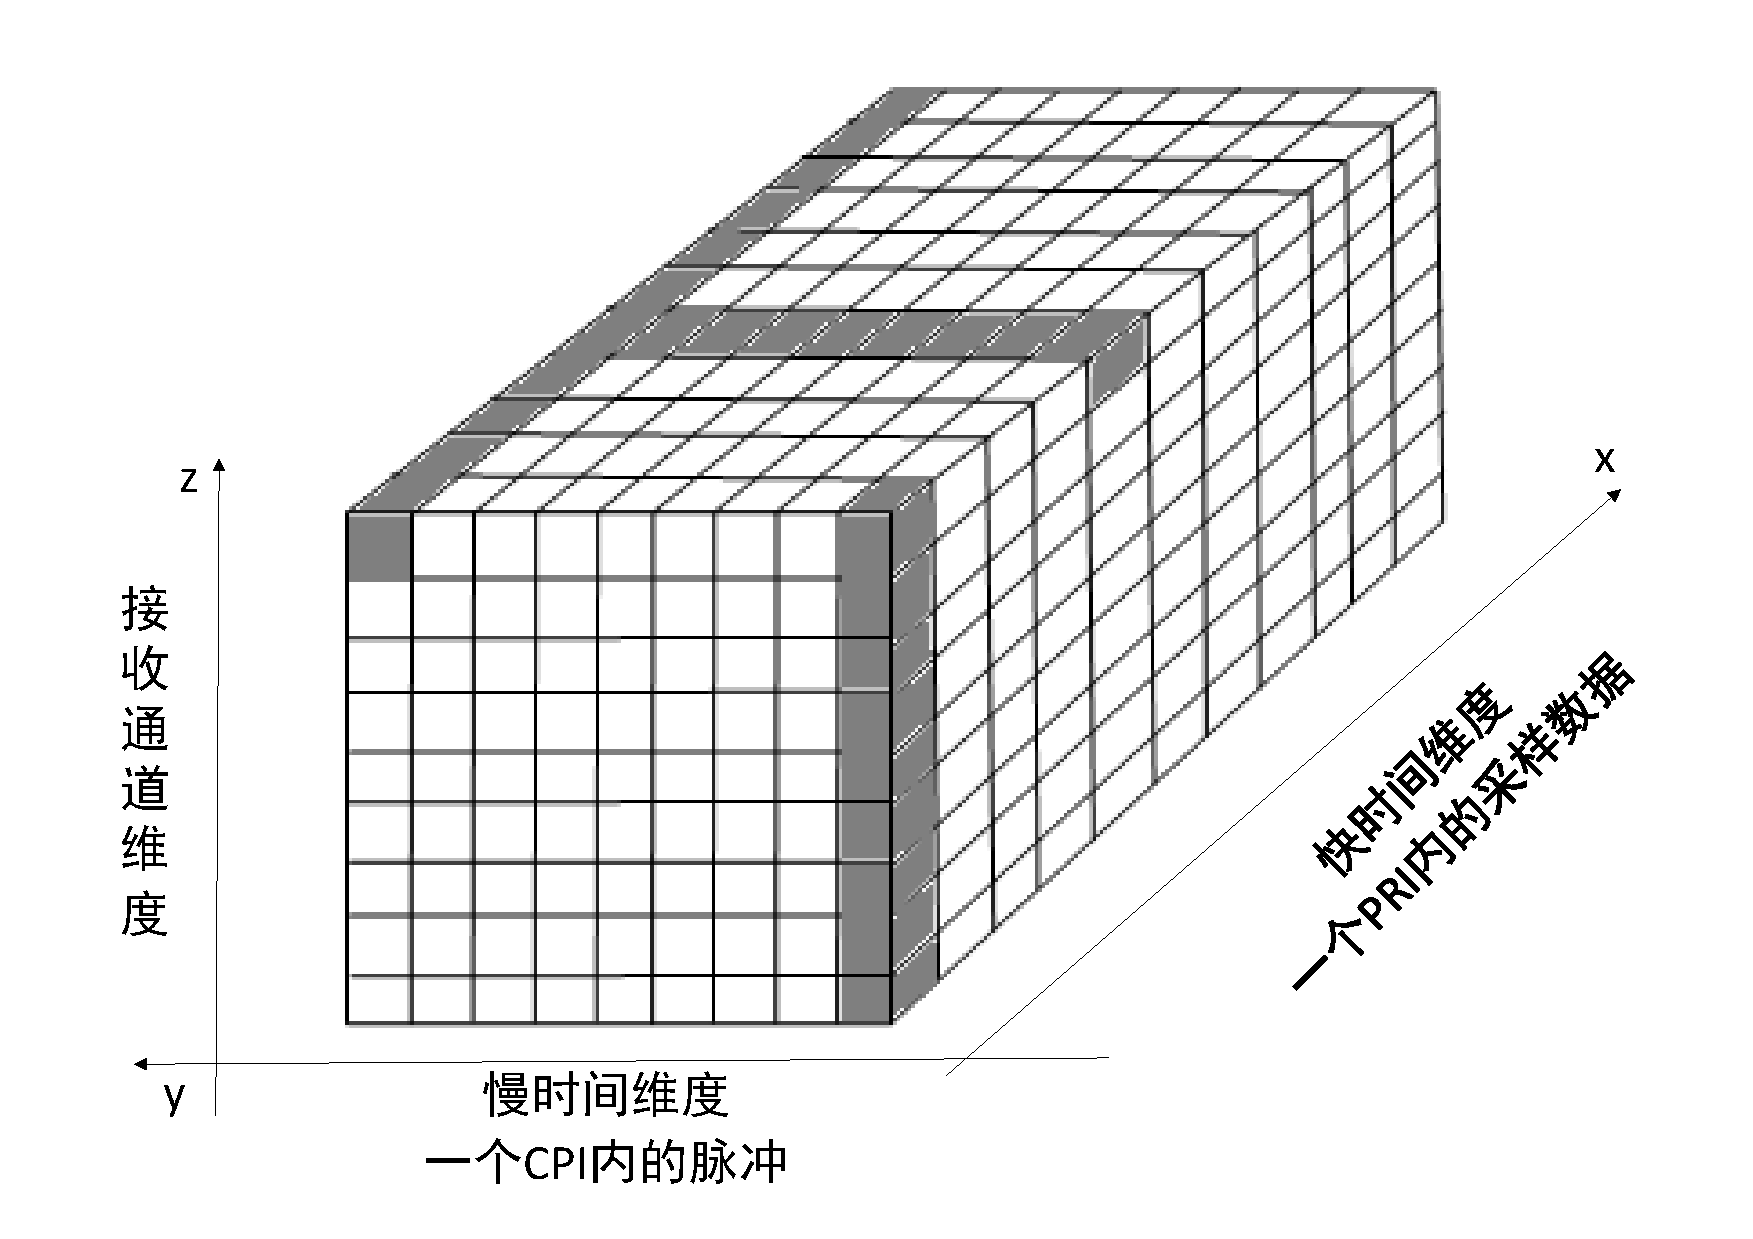
\includegraphics [width=1.0\textwidth]{figure//DataBlock.pdf}
    \caption{信号处理数据块}\label{DataBlock}
\end{figure}

可以看到,在上图中的x轴方向标注为快时间维度,本质就是一个PRI(脉冲重复间隔)内的回波
采样数据.y轴标注为慢时间维度,本质是一个CPI(相干处理间隔)内的多组回波数据。z轴标注的是
接收通道维度,本质就是对应天线的接收通道数目。

\subsection{数据模型理解}
上一节是介绍了基本的数据模型,在本节中还需要深入的理解一下设计的数据模型,在图2.2中,针
对数据模型的三个维度进行了进一步的标注。
\begin{figure}[hbtp]
    \centering
    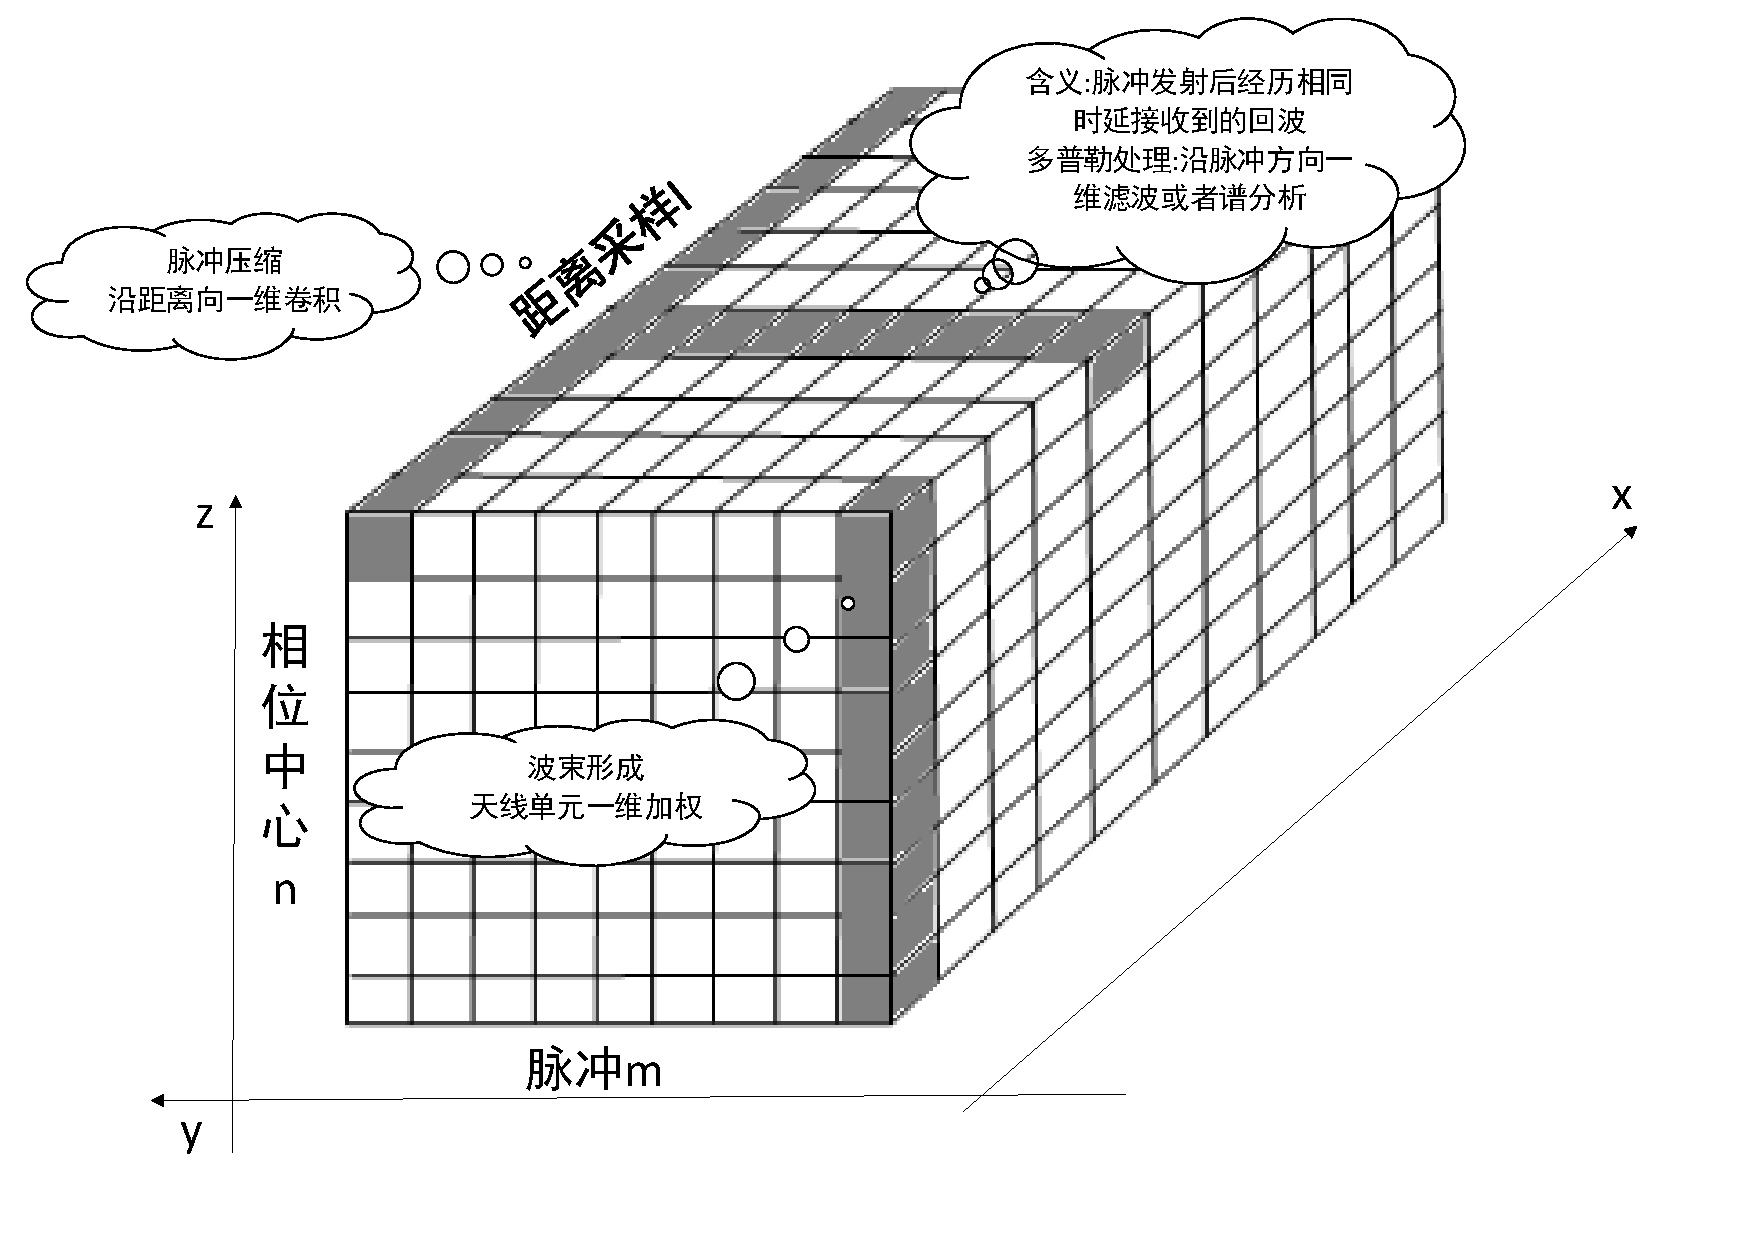
\includegraphics [width=1.0\textwidth]{figure//DataBlock2.pdf}
    \caption{信号处理数据块}\label{DataBlock2}
\end{figure}

x轴方向标注为距离采样l,脉冲压缩处理便是在这一维度做处理,而多普勒处理则是沿y轴方向,y轴
方向还有一个很重要的含义,便是脉冲发射后经历相同时延接收到的回波,z轴代表不同的接收通道,
不同的接收通道具有不同的相位,波束赋形便是在z轴方向来处理的。

在这里我们将一个接收通道的采样数据拿出来详细研究一下,如图2.3所示,将x轴和y轴方向的数据
转换到时间轴,一个距离库对应一个小方块,同时对应的就是一个采样周期内的采样数据,一列数据
便是一个PRT内采集到的数据,而一个CPI内的数据,则是多个PRT内的数据采集到一起进行数据处理。

\begin{figure}[H]
    \centering
    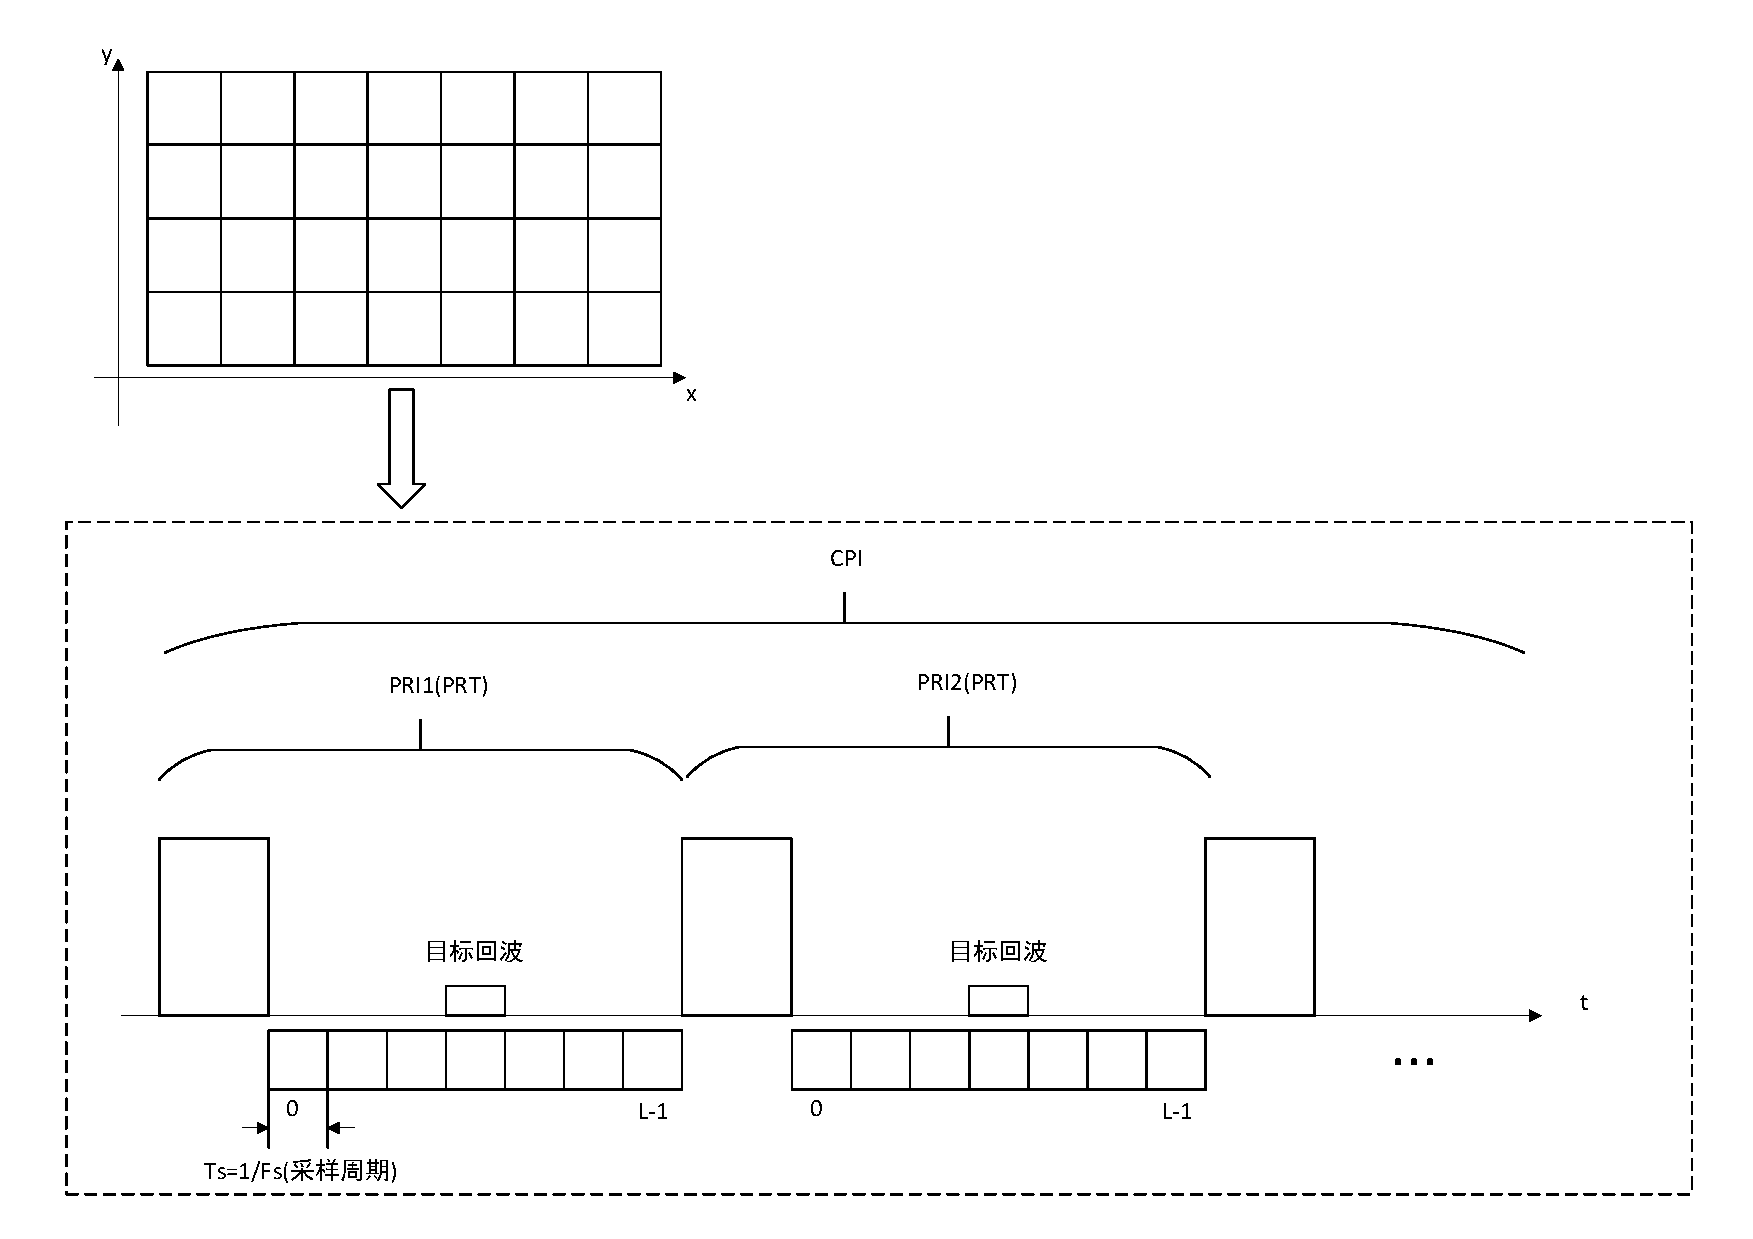
\includegraphics [width=1.0\textwidth]{figure//CPIdata.pdf}
    \caption{CPI数据}\label{CPIdata}
\end{figure}

根据上面两节的叙述基本建立了一个数据处理的模型,后面的计算和处理均会在这个三维模型来进行
展开。

\section{指标算法}
有了数据处理模型,还需要知道如何处理这个数据模型,现在就像做菜,菜的原材料已经有了,但是
还需要食谱,然后根据食谱做出想吃的菜,本节就是描述如何进行处理这些原材料。首先需要面对的
就是3个最基本的指标,反射率强度(Z),径向速度(V),速度谱宽(W),下面就逐个指标来进行计算,
其它指标后续逐步添加进入方案。

\subsection{反射率强度}
反射率强度(Z)是雷达回波的最基本指标,在这里主要引用
《雷达信号处理基础(第二版)》\cite{FundamentalsOfRadarSignalProcessing}中2.2.4节中的
计算模型,雷达气象学通常采用称为反射率的归一化因子来表示气象目标的散射特性,通常用Z表示,
体反射率(RCS)公式如下:

\begin{proposition}[体反射率]

    \begin{equation}
        \eta=\frac{\pi^5|K|^2}{\lambda}Z
    \end{equation}

    $|K^2|$:对于由水构成的散射体其值近似为0.93,由冰构成的散射体近似为0.197

    $\lambda$:雷达波长

\end{proposition}

当给出一个回波功率测量值,就可以用雷达方程估计出$\eta$,然后利用公式2.1换算成Z,再
对取10lgZ即得到dBZ。

《雷达信号处理基础(第二版)》\cite{FundamentalsOfRadarSignalProcessing}中2.2.2节给出
的体散射目标的雷达方程如下:
\begin{proposition}[体散射雷达方程]

    \begin{equation}
        p_r\left(t_0\right)=\frac{P_tG^2\lambda^2\eta\Delta R\theta_3\phi_3}{
                            \left(4\pi\right)^3R_0^2L_sL_a\left(R_0\right)}
    \end{equation}

    $p_r(t_0)$:$t_0$时刻回波接收功率

    $P_t$:雷达辐射功率

    $G$:天线增益

    $\lambda$:雷达波长

    $\Delta R$:一个距离分辨单元的长度

    $\theta_3$:方位3dB波束宽度

    $\phi_3$:俯仰3dB波束宽度

    $R_0$:分辨单元中心距离

    $L_s$:系统损耗因子

    $L_a(R_0)$:$R_0$处的大气衰减
\end{proposition}

根据公式2.1和2.2便可以解出Z,综合后的公式如下:
\begin{proposition}[体散射雷达方程]

    \begin{equation}
        Z=\frac{64}{\pi^2}*\frac{L_sL_a\left(R_0\right)}
            {P_tG^2\lambda|K|^2\Delta R\theta_3\phi_3}*R_0^2P_r(t_0)
    \end{equation}

\end{proposition}

根据公式2.3可以看出只要从上一节中的距离库获取$R_0$和$P_r(t_0)$便可以解出Z的值,公式中
的其它部分则可以根据相关的系统属性计算为一个常数。

$R_0$的值是比较好计算的,直接使用下面的公式:
\begin{proposition}[目标距离计算]

    \begin{equation}
        R_0=\frac{c*t_0}{2} 
    \end{equation}

    $c$:光速

    $t_0$:接收机接收回波的时间

\end{proposition}

下面重点介绍一下$P_r(t_0)$的计算,为了得到更好的信噪比,回波功率需要在一个CPI上来计算信
号功率,相干积累可以增加信噪比主要源于下面三个公式。

\begin{proposition}[相干积累]

    \begin{equation}
        \chi_1=\frac{A^2}{\sigma_w^2}
    \end{equation}

    \begin{equation}
        \sum_{n=0}^{N-1}\left\{Ae^{j\phi}+w\left[n\right]\right\}=NAe^{j\phi}+\sum_{n=0}^{N-1}w\left[n\right]
    \end{equation}

    \begin{equation}
        \chi_N=\frac{(NA)^2}{N\sigma_w^2}=N\chi_1
    \end{equation}

    $\chi_1$:单脉冲的SNR

    $A$:复回波$Ae^{j\phi}$的幅度值

    $\Sigma_w^2$:高斯白噪声的信号功率

    $w[n]$:噪声信号

    $\chi_N$:N个相干信号累计的SNR

\end{proposition}

根据相干积累公式中的原理,采样得到的总功率等于有效回波信号的功率加上噪声功率,而每个距离
库采样信号的值表示为I+jQ两路的数据,总功率可以通过$\sqrt{I^2+Q^2}$来计算。又根据相干积
累中信噪比可以提升N倍,这样有利于判断是否接收到的信号为有效的回波,当然为了计算接收回波的
功率,还需要计算噪声的功率。

噪声功率的计算方法:取最大俯仰角的接收通道,最远距离的256个距离库计算平均功率。

有了总功率和噪声功率,很自然便可以得到回波信号的功率$P_r(to)$。

\subsection{径向速度} 
径向速度的计算主要在慢时间维度(即数据块的y轴方向)进行处理,处理的原理主要是基于多普勒定律,
针对我司的气象雷达信号处理中多普勒处理主要有以下两个个方法:
\begin{enumerate}[1)]
    \itemindent=2em
    \item MTI(运动目标指示)
    
    \qquad MTI处理的目的主要是设计一个高通滤波器滤除杂波,如图2.4所示,

    \begin{figure}[hbtp]
    \centering
    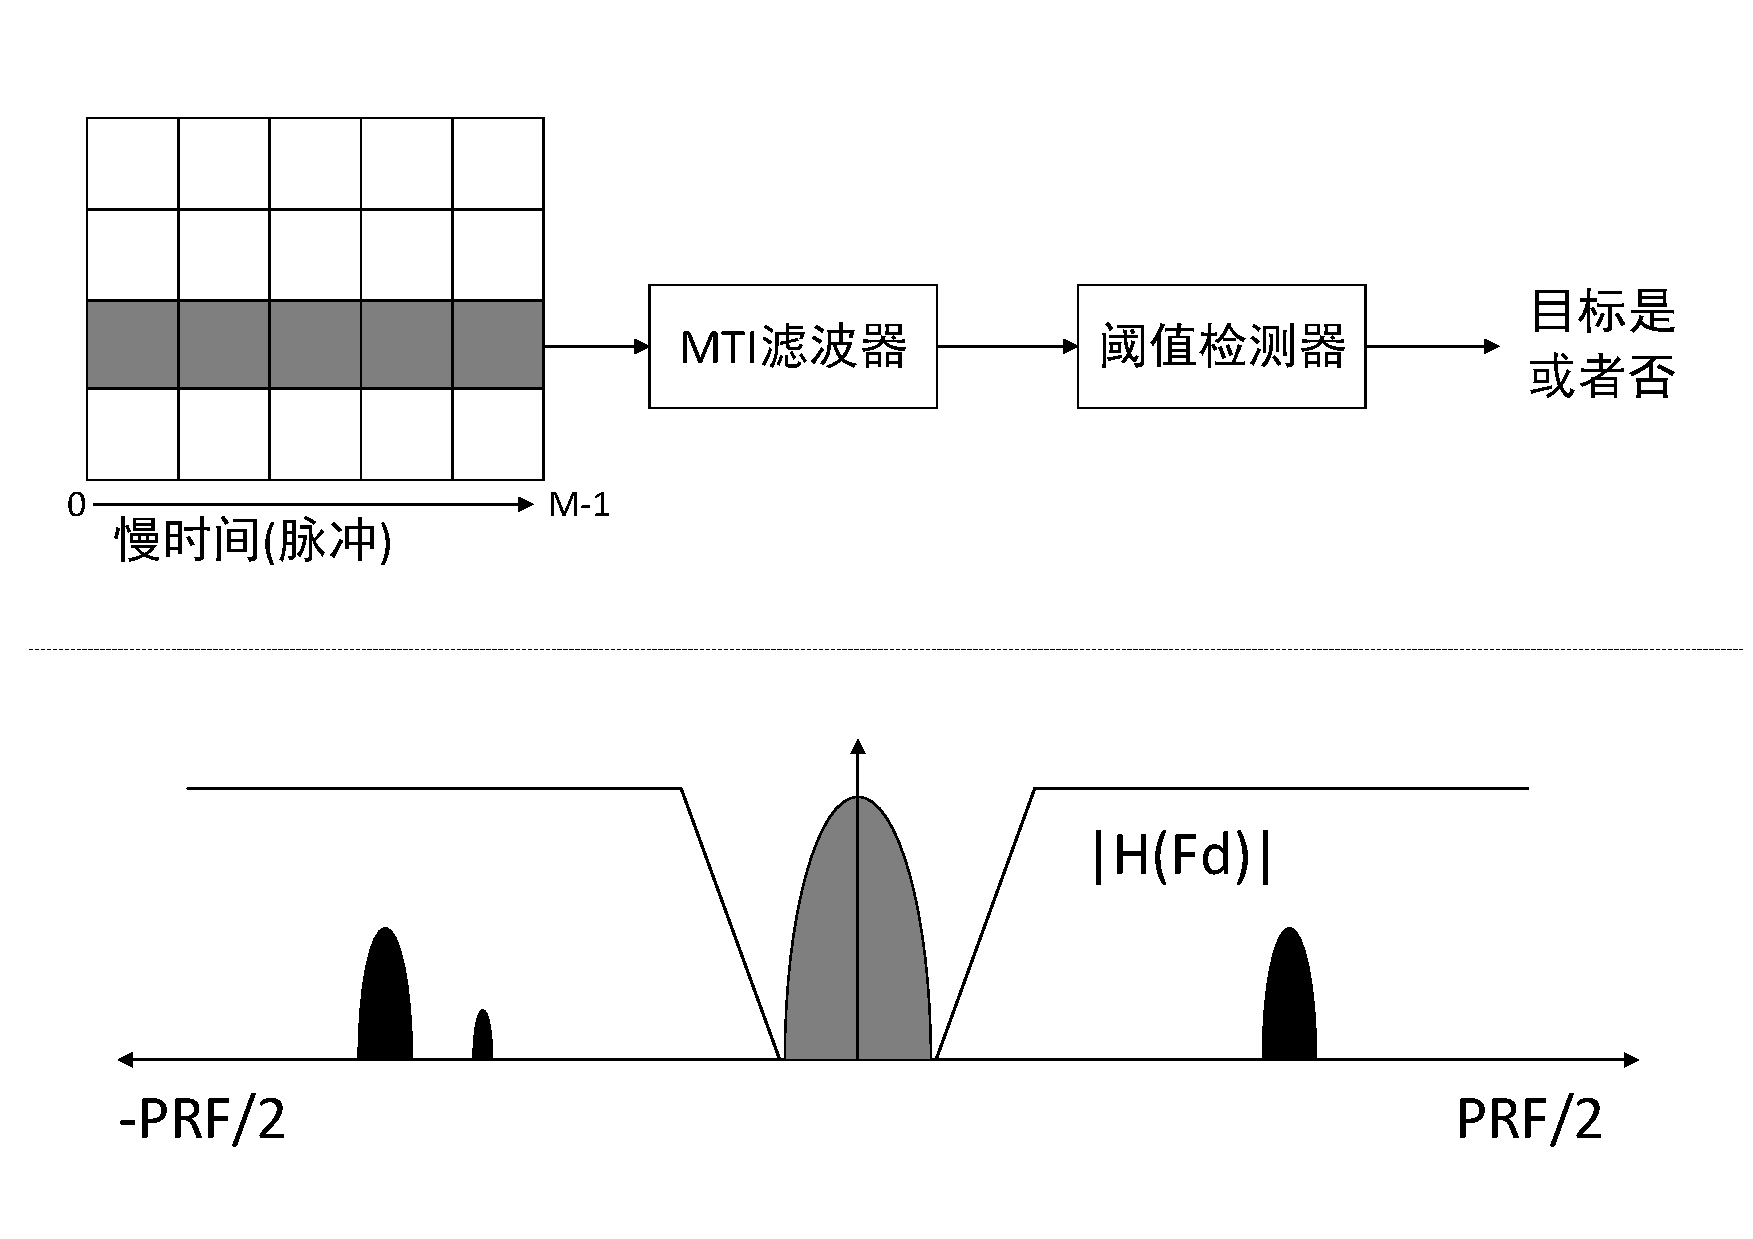
\includegraphics [width=1.0\textwidth]{figure//MTI.pdf}
    \caption{MIT处理}\label{MTI}
    \end{figure}

    \item 脉冲对处理(PPP)\cite{FundamentalsOfRadarSignalProcessing}\cite{radarmeter}
    \cite{RadarManual}
    
    \qquad 在气象雷达中脉冲对处理主要是为了计算目标谱峰的参数,速度计算如公式6
    所示,处理原理主要是依据目标速度比较慢,频谱偏移比较小,采用计算相位的办法更为合适,
    具体的阐述可以看引用网页\cite{dopler.web},在上面做了比较清晰的解释。

    具体的推导原理就是根据图2.5。
    \begin{figure}[hbtp]
        \centering
        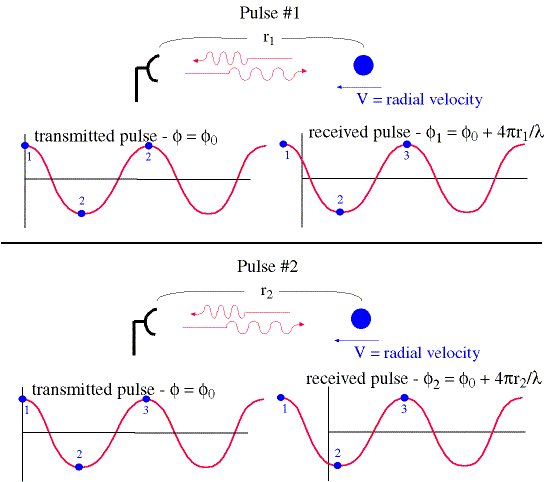
\includegraphics [width=1.0\textwidth]{figure//pulse.png}
        \caption{相位计算}\label{pulse}
    \end{figure}

    根据图中所示,做如下推导:

    \begin{proposition}[相位计算推导公式]
        
        \begin{equation}
            \phi = \phi_0 + \frac{4\pi r}{\lambda}
        \end{equation}

        $\phi_0$:发射信号的相位

        $\phi$:接收信号的相位

        等式两边做微分可得:

        \begin{equation}
            \frac{d\phi}{dt}=\frac{4\pi}{\lambda}\frac{dr}{dt}
        \end{equation}

        $dt$:dt就是两个采样之间的时间间隔T

        $\frac{dr}{dt}$:就是速度V

        \begin{equation}
           V=\frac{\lambda}{4\pi T}d\phi
        \end{equation}

    \end{proposition}

    在这里主要希望计算的是相位的变化。

    \begin{proposition}[速度计算公式\cite{RadarManual}]

    \begin{equation}
        R[T]=\frac{1}{N}\sum_{k=0}^{N-1}s[k+1]s^*[k]
    \end{equation}

    \begin{equation}
        V_0=\frac{\lambda}{4\pi T}arg\left\{R(T)\right\}
    \end{equation}

    $R(T)$:相邻两个脉冲的自相关函数

    $s_k$:复通向(I)和正交(Q)信号样本

    $V_0$:径向速度

    $P_n$:噪声功率

    $T$:连续两次取样的时间间隔

    $\lambda$:波长

    \end{proposition}

\end{enumerate}

\subsection{速度谱宽}

计算出径向速度之后,也可以使用自相关函数计算出谱宽,谱宽计算在这里直接采用雷达手册中给出
的公式,如公式7所示。

    \begin{proposition}[谱宽计算公式\cite{RadarManual}]

    \begin{equation}
        \sigma^2\approx\frac{\lambda}{8\pi^2 T^2}arg\left\{1-\frac{R(T)}{R(0)-P_n}\right\}
    \end{equation}

    $R(T)$:相邻两个脉冲的自相关函数

    $R(0)$:相当于将自己与自己的复共轭相乘之后除以N

    $s_k$:复通向(I)和正交(Q)信号样本

    $V_0$:径向速度

    $T$:连续两次取样的时间间隔

    $\lambda$:波长

    \end{proposition}

\end{spacing}

%---------------------------------------------------------------------
%  第三章 模块设计
%---------------------------------------------------------------------
\chapter{设计实现}
\begin{spacing}{1.5}
\songti\zihao{-4}

上一章主要讨论了雷达回波几个关键参数的处理原理,这一章主要讲的是结合硬件设备的软件实现。
首先需要考虑的问题便是数据的获取,其次便是如何处理数据。
\section{数据获取}
\subsection{数据接收}
在第一章的硬件框图中可以看到,x86板主要通过PCIe接口从FPGA接收数据,接收数据的过程中,主
要需要考虑的就是接受的数据的数据量大小,而接收数据量大小又和发射脉冲、接收通道等有关,下
面列出了一个单通道一个CPI数据量评估公式:

    \begin{proposition}[数据量算公式]

    \begin{equation}
        Data=4L_{dist}*C_{prt}+C_{prt}*H
    \end{equation}

    $4$:表示需要4个字节用来存放IQ两路采样数据

    $L_{dist}$:距离库数目,根据探测距离决定

    $C_prt$:PRT个数,在我司研发的系统中采用的是64个PRT

    $H$:每个距离库的头部信息字节数

    \end{proposition}

这里可以大概根据公式评估数据量,假设$L_{dist}$值为1500,H为64字节,则大致可以计算出一个
CPI内单通道数据为379KByte。

目前PCIe驱动已经完成了调试,接收数据通道目前基本已经打通。

\subsection{数据存储}
完成数据的接收之后,主要考虑的是数据要按照计算要求进行存储,以便于进行数据处理。讨论
到计算处理,需要先来看一下计算部分的物理结构。根据之前的计划,是采用GPU卡来加速信号处理计
算,目前所使用的GPU卡内部结构基本如图3.1\cite{CudaGuide}所示:

\begin{figure}[hbtp]
    \centering
    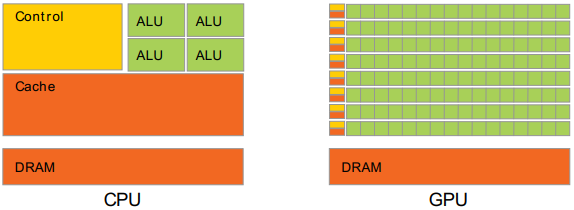
\includegraphics [width=0.8\textwidth]{figure//GpuStruct.png}
    \caption{GPU结构}\label{GpuStruct}
\end{figure}

GPU有独立的内存和网状结构的个内部处理单元可用于并行处理,基本的结构如图3.2所示,一个小
方块就是代表一个处理单元叫做 Streaming Multiprocessors(SMs)。    

\begin{figure}[hbtp]
    \centering
    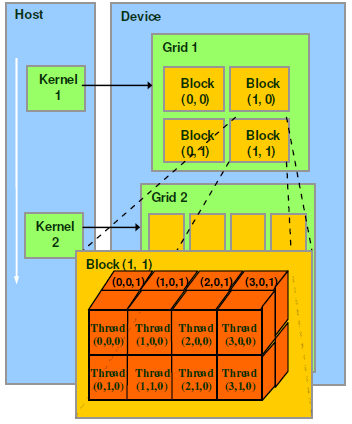
\includegraphics [width=0.5\textwidth]{figure//block.png}
    \caption{GPU并行处理单元}\label{block}
\end{figure}


为控制GPU的并行计算处理,Nvidia推出的Cuda对底层物理硬件做了封装,从软件角度来看,并行计
算单元主要划分为block和Thread,每个block会分配到不同的SMs上执行,并行处理的一个主要的方
面就是分配Block和Thread的索引。

关于GPU另外一个需要了解的部分就是GPU的内存体系结构,GPU内部内存支持多种的的模式,具体如
图3.3所示,包括local memory是一个Thread的本地内存,shared memory是一个Block共享的内存,
而Global memory是全局共享的内存。

\begin{figure}[hbtp]
    \centering
    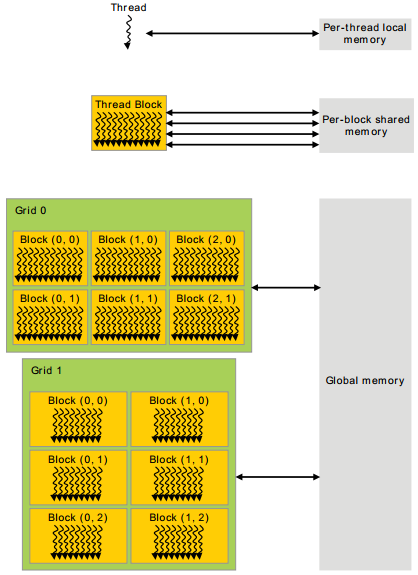
\includegraphics [width=0.4\textwidth]{figure//memory.png}
    \caption{GPU内存体系结构}\label{memory}
\end{figure}

上面基本介绍了GPU的体系结构之后,结合雷达信号处理的特点,使用GPU来计算处理雷达数据还是比
较合适的。在上一章的雷达数据模型的计算中已经描到,针对数据模型的处理主要是按照距离库划分,
在慢时间维度的数据处理可以分配到每一block进行处理。

\begin{figure}[H]
    \centering
    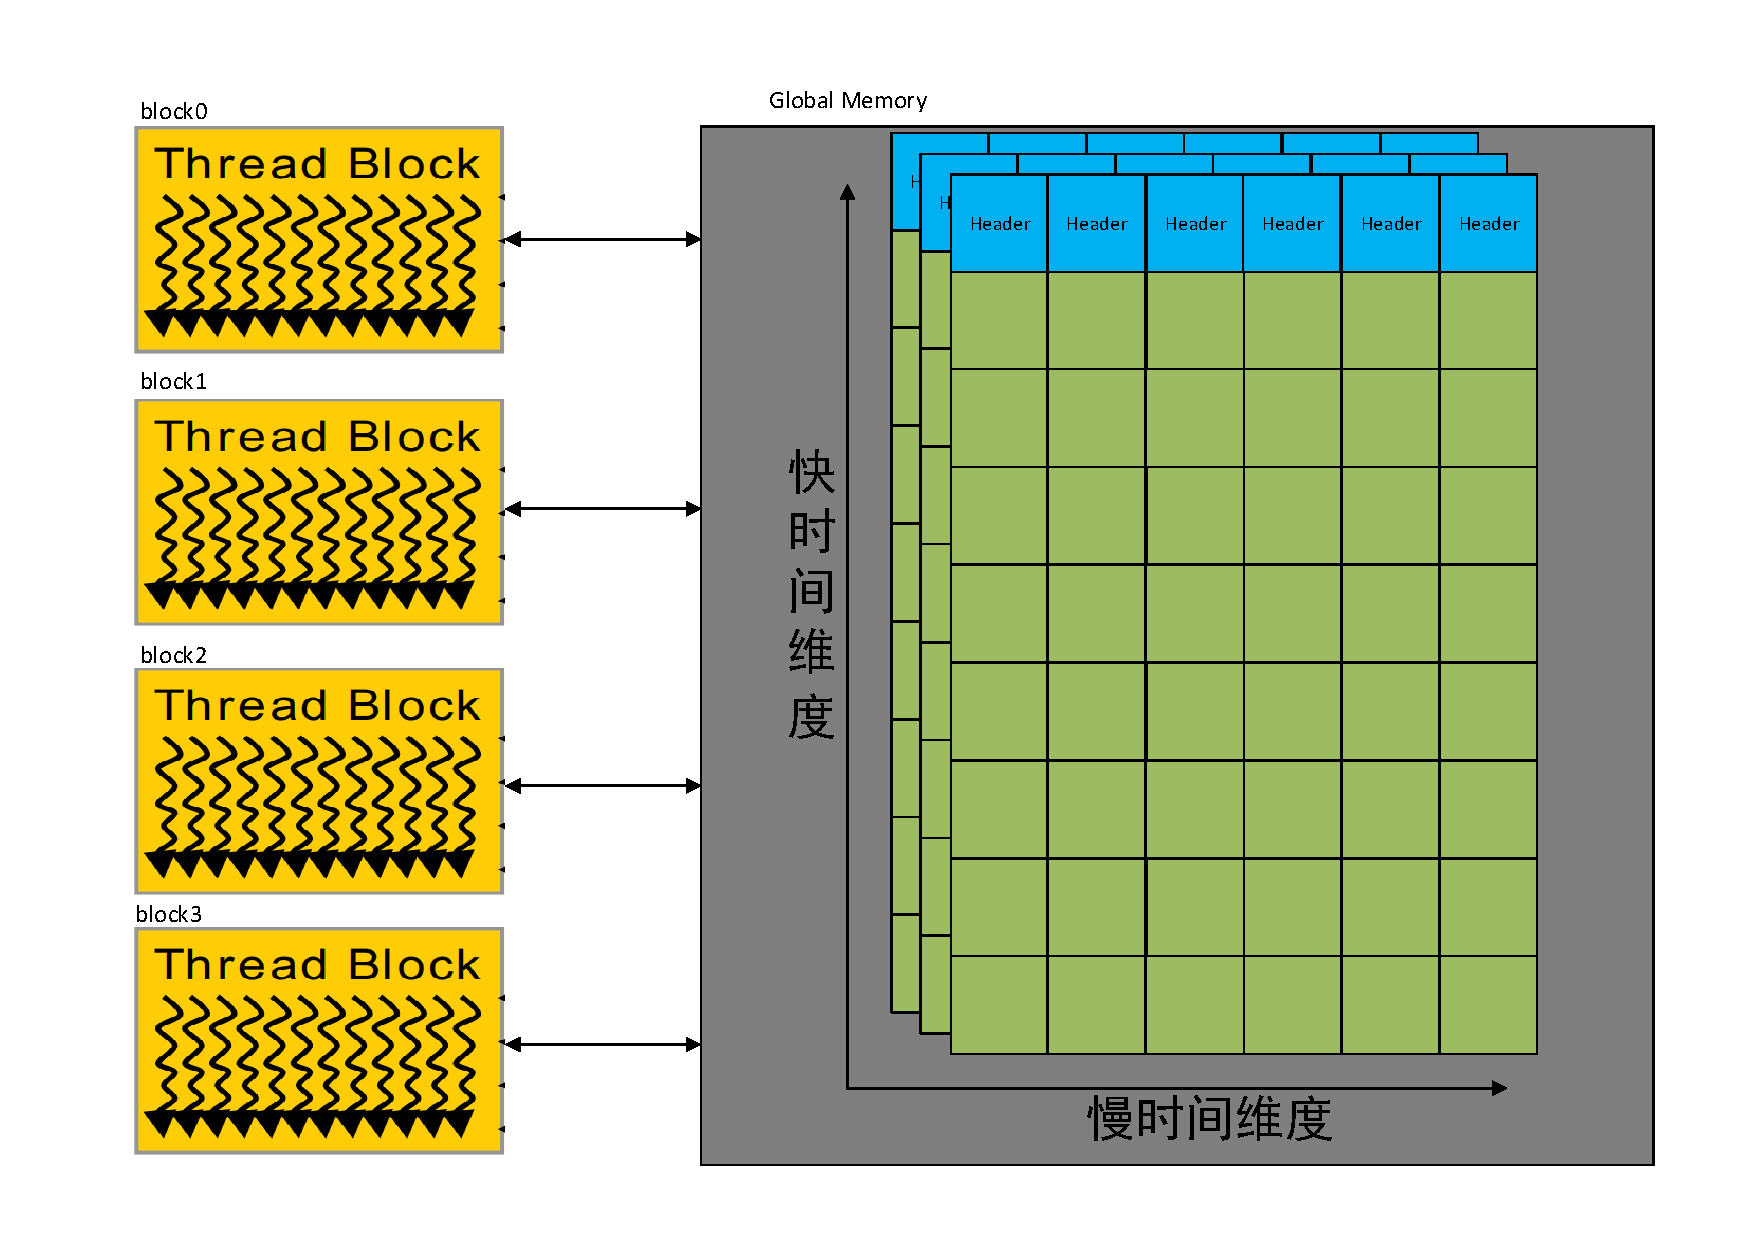
\includegraphics [width=0.7\textwidth]{figure//DataCache.pdf}
    \caption{数据存储}\label{DataCache}
\end{figure}


根据GPU的内存模型,最好的方法便是在GPU的Global Memory建立一个全局的数据矩阵,数据矩阵的
格式便是安照雷达数据处理模型来存储,具体的存储模型如图3.4所示进行划分。

\section{数据处理}
数据处理这一节主要是根据上一章整理的雷达信号处理的算法进行设计实现。上一章描述了主要的计
算目标就是雷达回波强度、径向速度和谱宽的计算,根据算法的描述基本的计算流程可以如下图3.5
所示。

\begin{figure}[htbp]
    \centering
    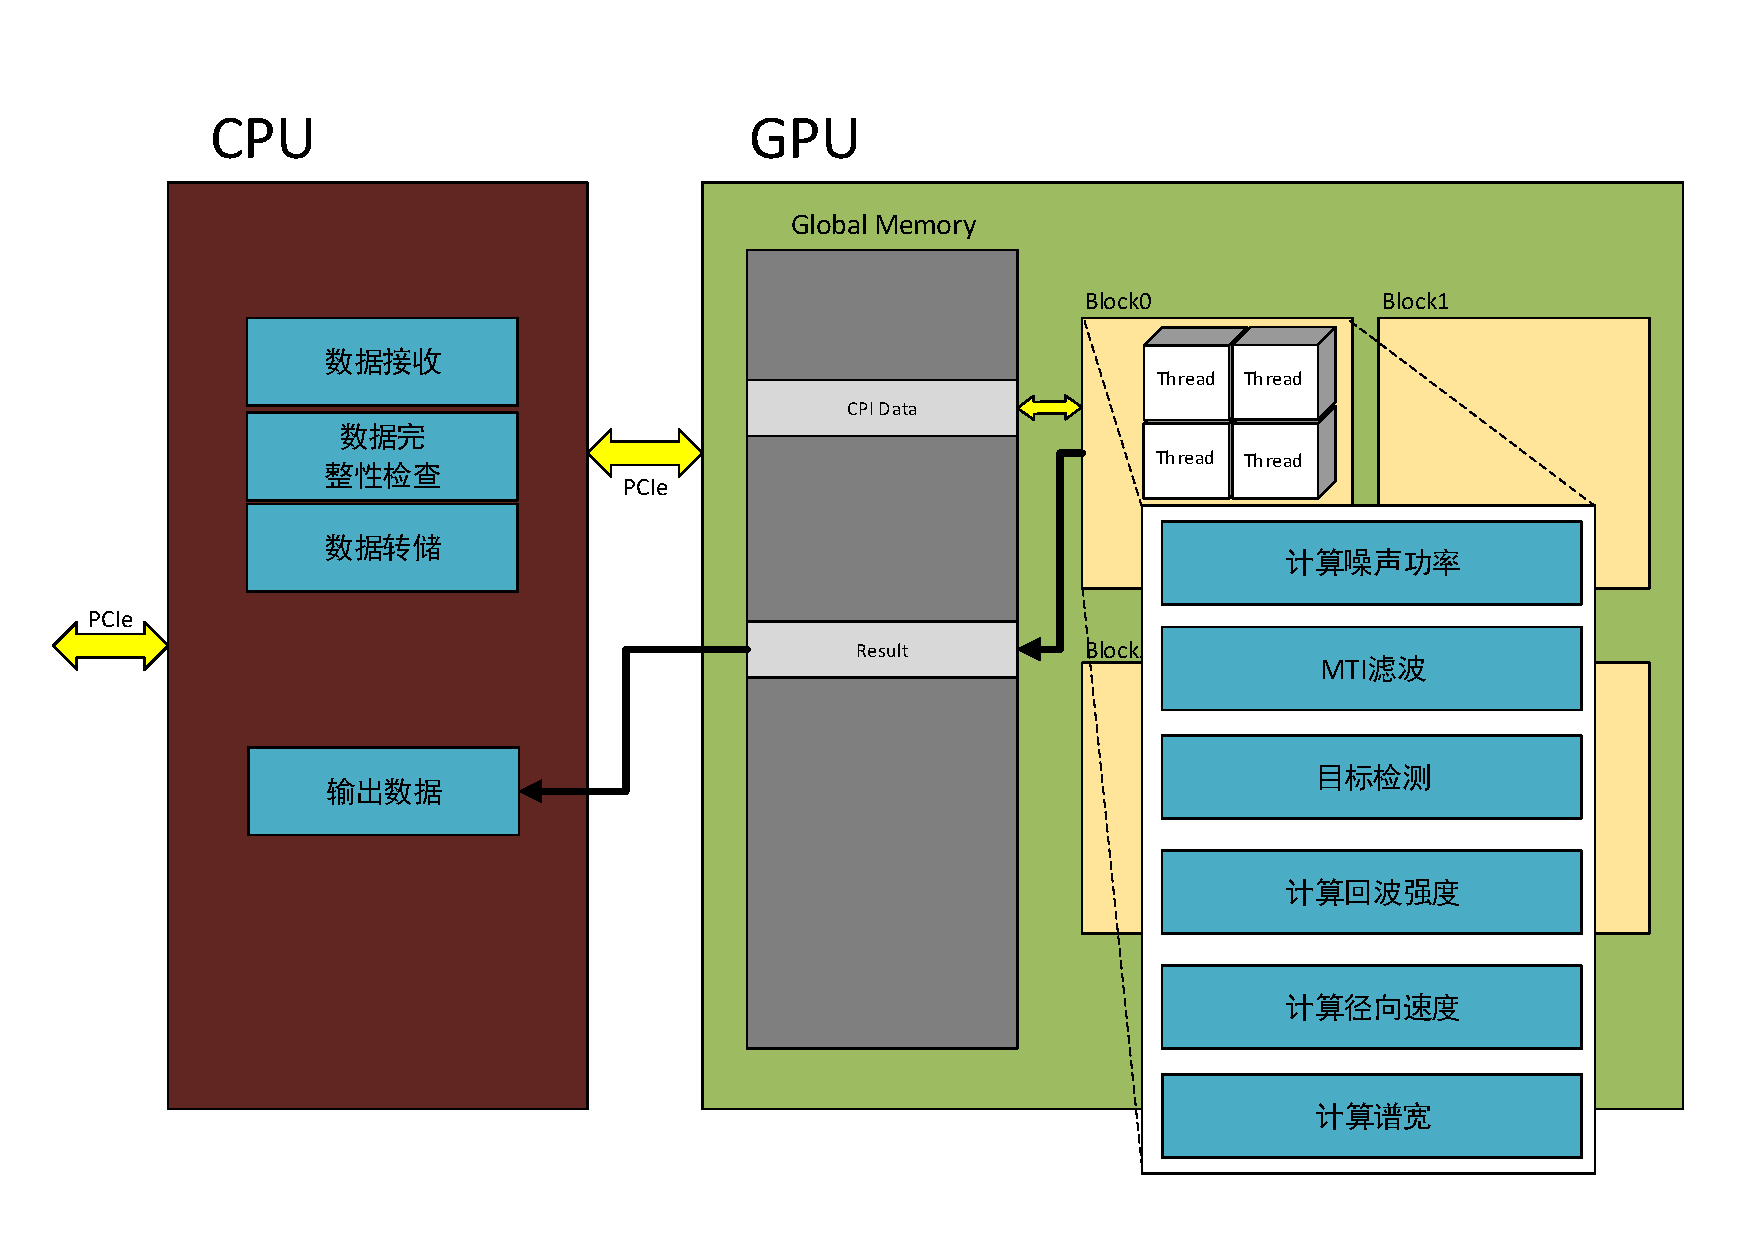
\includegraphics [width=1.0\textwidth]{figure//countflow.pdf}
    \caption{处理流程}\label{countflow}
    \end{figure}
\end{spacing}

在CPU一侧主要需要做的处理为数据接收,数据接收处理负责通过PCIe驱动从FPGA接收数据包,数据
完整性检查处理负责检查每一包数据各项参数是否完整正确,数据转储处理负责将数据从CPU转储到
GPU全局内存区,同时如果出现GPU内存区数据溢出的情况下,可以在数据转储处理中做一个数据缓冲。

GPU一侧的计算则主要负责算法的并行计算,首先做的便是提取回波噪声功率用于后续计算的使用,然
后是进行MTI滤波,滤除杂波的处理可以让后续的计算结果更加精确可靠。计算回波强度、计算径向速
度和计算谱宽的处理则可以并行进行。

%---------------------------------------------------------------------
%  第四章 详细设计
%---------------------------------------------------------------------
\chapter{详细设计}
\begin{spacing}{1.5}       

\section{协议设计}
本节主要设计了FPGA与上层x86平台的数据包格式,数据包中包含计算处理过程中需要的数据和相关
参数,具体格式如图4.1所示,使用64个字节作为报文头,数据区则根据距离库的大小进行设计。

\begin{figure}[htbp]
    \centering
    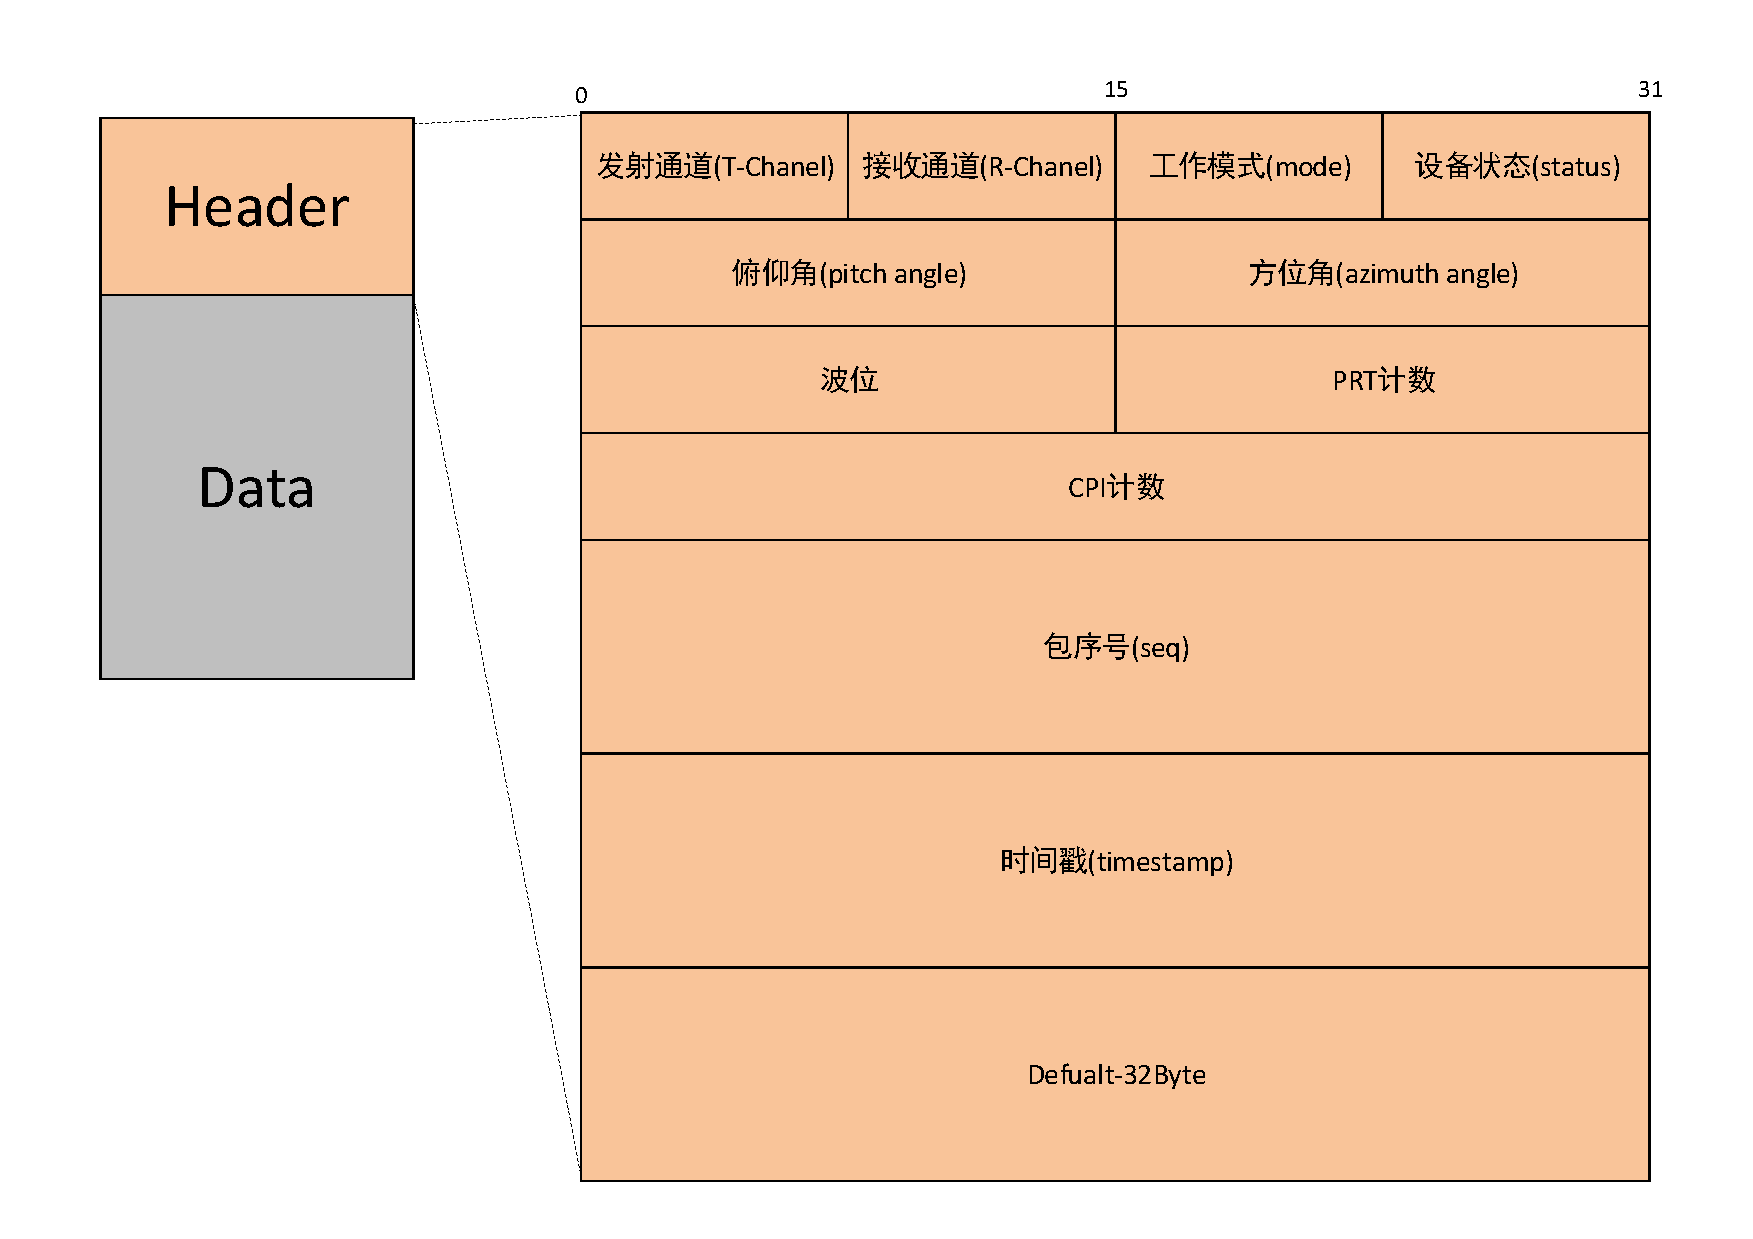
\includegraphics [width=1.0\textwidth]{figure//header.pdf}
    \caption{协议包格式}\label{header}
\end{figure}

目前格式只是暂定,具体的格式还需要根据结合FPGA进行详细讨论。

\section{软件框架}
本节主要根据GPU软件设计模型,设计了基本的软件处理框架用于指导后续的代码编写过程。
\begin{figure}[htbp]
    \centering
    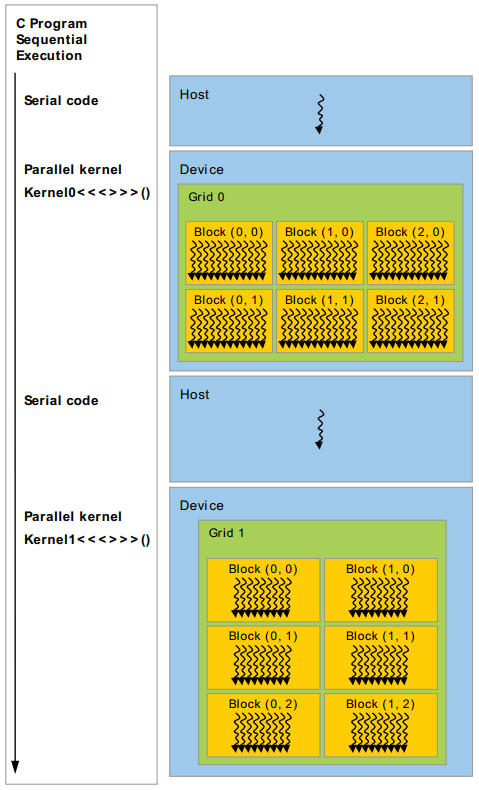
\includegraphics [width=0.5\textwidth]{figure//softflow.png}
    \caption{软件设计模型}\label{softflow}
\end{figure}

在Cuda官方提供的编程指导\cite{CudaGuide}中提供了一个基本的编程模式,具体如图4.2所示,
在雷达信号处理的代码中也将遵循这个基本编程模型。

按照基本编程模型设计的软件程序框架如图4.3所示,程序启动之后需要完成对FPGA的初始化,如果
初始化失败则退出程序。

完成FPGA初始化之后,开始进行数据接收,完成一个数据块的接收之后进行数据有效性检查,确定
数据为有效数据,然后开始数据的转储,由CPU内存转储到GPU内存,如果GPU内存已经接近溢出,则
转储处理还需要进行数据缓存,同时完成数据转储之后还会同步需要进行数据接收。同时程序会检查
GPU内存中的数据是否已经存储完成,一旦完成存储立即开始启动并行计算,计算相应的回波噪声功率,
对同一个距离库的程序进行滤波处理,完成滤波处理之后进行目标检测,根据目标检测结果决定是否
进行相关的参数计算。

\begin{figure}[hbtp]
    \centering
    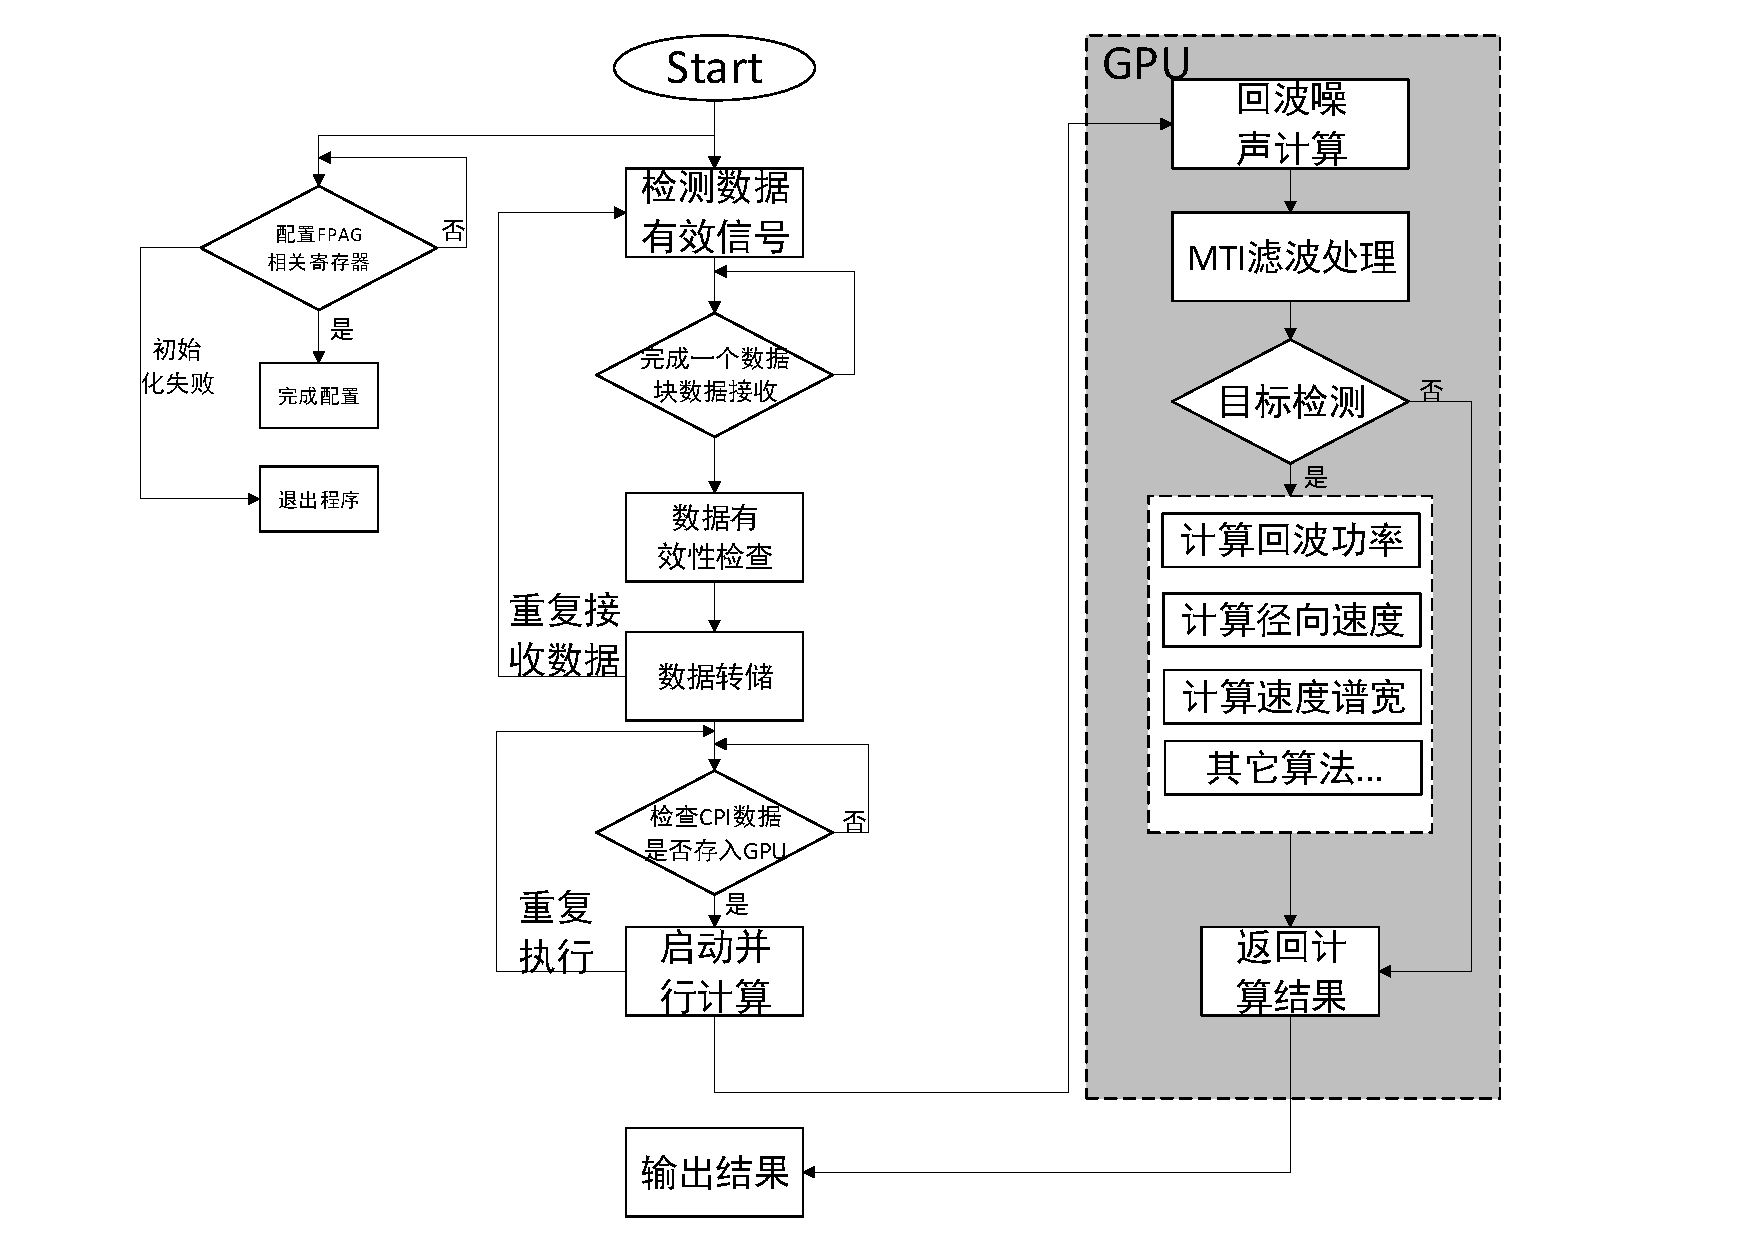
\includegraphics [width=1.0\textwidth]{figure//softflow.pdf}
    \caption{软件设计框架}\label{softflowpdf}
\end{figure}

如果检测到有目标,则计算回波功率、计算径向速度、计算谱宽,这三个值可以并行计算,算法部分
的设计将会设计成模块化的模式,每一种算法均可方便进行添加删减,这样便于后续添加更加高级的
算法处理模块,在完成计算之后,GPU一侧的程序将会将计算结果输出到CPU主机一侧。

\end{spacing}
%---------------------------------------------------------------------
%  第五章 总结
%---------------------------------------------------------------------
\chapter{总结}
\begin{spacing}{1.5}       
雷达信号处理部分相关内容比较多且复杂,我司又缺少雷达信处的设计实现经验,并且从理论算法到
工业实现,整个过程只能在摸索逐步实现,本方案也只是一个初步的讨论方案,但是只要一步一步讨
论清楚,集思广益,则定能从无到有,从有到优。
\end{spacing}

%---------------------------------------------------------------------
%  参考文献设置
%---------------------------------------------------------------------
\addcontentsline{toc}{chapter}{参考文献}

\begin{thebibliography}{99}
\songti \zihao{-4} 	
    \bibitem{FundamentalsOfRadarSignalProcessing}
    Mark A.Richards . 雷达信号处理基础 (第二版) [M]. 2008.
    \bibitem{radarmeter}
    张培昌. 雷达气象学[M]. 气象出版社, 1988.
    \bibitem{dopler.web}
    http://apollo.lsc.vsc.edu/classes/remote/lecture\_notes/radar/doppler/two\_pulses.html
    \bibitem{RadarManual}
    斯科尼克(Skolnik,M.I.) 雷达手册: 第3版/(美) 南京电子研究所, 2010.
    \bibitem{CudaGuide}
    CUDA C PROGRAMMING GUIDE, October 2018.

\end{thebibliography}

\end{document}